The goal of numerical techniques is to simulate the physics of real world systems. These are, to some extent, captured by different models. Models are a simplified mathematical description that captures some relevant physics of more complicated systems. This section introduces some specific models, their relevance and some properties. These models will be used later to benchmark the developed tensor network expansion.

\subsection{Ising model}

The prototypical example of a model in the field of strongly correlated matter is the Ising model. It was first introduced 1925 by Ernest Ising, as a model to capture ferromagnetism. He proved that for a linear chain, there is no phase transition at finite temperature. He wrongly concluded that this would also be the case in higher dimensions, but it turned out t be one of the deepest and far-reaching problems in 20th century \cite{Taroni2015}.

The Ising model, in essence, assigns an energy contribution to neighbouring spins. These spins sit on a fixed position on a chain (1D) or lattice (2D/3D/...). In classical Ising, the operators in the Hamiltonian all commute with each other. An energy is assign between neighbouring spins and possible and energy for alignment with an external magnetic field in the same direction. In quantum Ising model, a transversal field is added. Often, the particles on the grid are spin 1/2 particles, but of course other particles are possible.

Many generalizations exist for the Ising model. \todo{q potts,...}

\subsubsection{Classical Ising}

The classical Ising model is given by the following hamiltonian:
\begin{equation}
    H = -J \left (  \sum_{<i j>} \sigma_i \sigma_j + h \sum_i \sigma_i \right )
\end{equation}
where $<i j>$ runs over all neighbouring lattice sites. The possible values of $\sigma$ depends on the spin dimension. For spin $1/2$ lattices $\sigma \in {-1,+1}$. g encodes the interaction strength of the external magnetic field.

The sign J determines the low temperature ground state. A positive J will tend to align all neighbouring spins at low temperature. This is often called ferromagnetic, because all the aligned spins cause a macroscopic magnetisation. On the other hand, a negative J causes neighbouring spins to have an opposite sign.

Depending on the sign of the longitudinal field h, the spins tend to align or anti align with this external field. This lifts the degeneracy of the ground state.

\paragraph{1D}

The classical 1D model was solved analytically by Lens. \todo{blabla}

\paragraph{2D}

In 2D, it becomes important to define the lattice. Here, and in the simulations, we will consider a square lattice. This model was famously solved by Lars Onsager in 1944, by using the transfer matrix method. In 2 dimensions, the Ising model has a phase transition at finite temperature. The critical temperature is $T_c = \frac{2 J}{T ln( \sqrt{2}+1)}$.

Only the $h=0$ case the is solved analytically. For higher dimensions, no analytical solution is known. For these cases, we need to use numerical techniques if we want to understand the behaviour of these models.

On different lattices, interesting thins can happen. For instance, the ground state of an antiferromagnet on a triangular lattice is not obvious to determine. The spins tend to antialign, but at least 2 of 3 spins on the corner of a triangle have to align. Remarkably, as will be explained in \cref{sec:PhasesAndCrit}, the physics at the phase transition does remain invariant when the lattice is changed.

\subsubsection{Quantum Ising}

As we all know, the real world behaves, certainly at small length and time scales, quantum mechanically. Therefore, it is important to understand how the quantum Ising model differs from the classical model. In the quantum Ising model, the operators no longer commute with each other. An example is the transversal Ising model given by the following hamiltonian:

\begin{equation}
    \hat{H} = -J \left (  \sum_{<i j>} \sigma^x_i \sigma^x_j + g \sum_i \sigma^z_i \right )
\end{equation}

In the case that $g=0$, this is the classical Ising model (in the $h=0$ case).

\paragraph{1D}
Different to the classical case, the 1D model already contains a phase transition.

\paragraph{2D}

\begin{figure}
    \center
    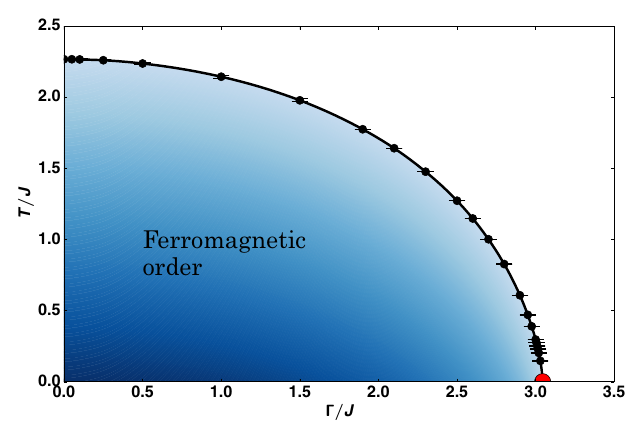
\includegraphics[width=\textwidth]{Figuren/phsyics/2disingphase.png}
    \caption{Phase diagram for 2D transversal Ising model. Figure taken from \cite{Hesselmann2016}.}
    \label{2dtisingphasediag}
\end{figure}

\subsection{Heisenberg}

The heisenberg model is given by:

\begin{equation}
    \hat{H} =  -\left( \sum_{<i j>} J_x \sigma^z_i \sigma^z_j + J_y \sigma^y_i \sigma^y_j+ J_z \sigma^z_i \sigma^z_j + h \sum_i \sigma^z_i \right )
\end{equation}

These models have different names depending on the values of $J_{\alpha} $ with $\alpha=x,y,z$. $J_x = J_y \neq J_z = \Delta$ is called the XXZ model.

\subsection{Random}
It's also possible to construct random hamiltonians. \todo{in basis: hermitian H}

\subsection{Quantum to classical mapping}

In a certain sense, a quantum model in d dimensions can be mapped to a classical model in d+1 dimension.

Due to the Lie product formula
\begin{equation}
    e^{A+B} = \lim_{M \to \infty } ( e^{A/M} e^{B/M}  )^M
\end{equation}
we can rewrite
\begin{equation}
    \begin{split}
        Z &= \sum_n e^{ - \beta E_n} \\
        &= \sum_n \Braket{n | e^{ - \beta \hat{H} }  | n} \\
        &= \sum_{n_1 \cdots n_M} \Braket{n_1 | e^{ - \beta \hat{H} /M}  | n_2}  \Braket{n_2 | e^{ - \beta \hat{H} /M }  | n_3} \cdots  \Braket{n_{M} | e^{ - \beta \hat{H} /M }  | n_1} \\
        &= \sum_{  n_1 \cdots n_M} \Braket{n_1 | e^{ - \beta \hat{H} /M}  | n_2}  \Braket{n_2 | e^{ - \beta \hat{H} /M }  | n_3} \cdots  \Braket{n_{M} | e^{ - \beta \hat{H} /M }  | n_1} \\
    \end{split}
\end{equation}
Where completeness relations $ I = \sum_{n_i}  \ket{ n_i } \bra{ n_i}  $ inserted M times in line 3. This is similar to a path inegral.

The quantum imaginary time has become a spatial dimension. The quantum model of d dimensions now has the structure of a classical model in d+1 dimensions.

In this way, the 2D transversal field ising model can be mapped to the 3D classical Ising model. \cite{Hsieh}